\chapter{Background \& Objectives}

\section{Problem Description}

The Travelling Salesperson Problem (TSP) is tasked with solving the problem "Given a list of cities and the distances between each city what is the shortest possible route that visits each city once and then returns to the origin city". This shortest route is called a Hamiltonian Cycle and has many applications such as in the fields of logistics, route planning and manufacturing\cite{acobook}. Dantzig, Fulkerson and Johnson were the first people to attempt to solve TSPs through the use of branch and bound\cite{dantzig1954solution}, the time taken to solve TSPs through this method was too high to be practical so since then TSPs have attempted to be solved through the use of many new intuitive algorithms.

Every method to solve TSPs has a limit on the size of problems that it can solve because it would simply take too long to solve problems above a given size. My project is a way of solving TSPs through the use of clustering and an Ant Colony Optimisation (ACO) Algorithm.

There are many freely available data sets of TSPs I have used the ones provided by The University of Waterloo\cite{tsp_test_data_2009} these are all of varying sizes and complexity and are provided in the common TSPLIB95 format, they also all have their optimal solutions noted so that easy comparisons can be made and so I can see how my algorithm performs. This TSP data is split into two main categories National (World) and VLSI, world test data is based on cities on a map and range in size from 29 nodes to 71,000 nodes, VSLI data is based on solder points in circuit boards. These two types of problems look very different and will require different types of clustering algorithms to properly solve. Figure \ref{fig:vlsi_tsp_data} shows VLSI test data and figure \ref{fig:world_tsp_data} shows an example of a world TSP problem.

\begin{figure}
    \centering
    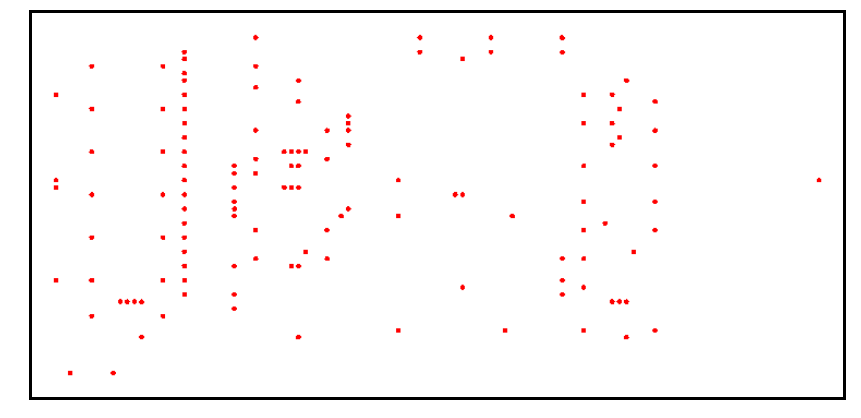
\includegraphics[width=\textwidth]{figures/vlsi_xqf131_tsp_data.png}
    \caption{Figure showing VLSI TSP test data, the nodes in this problem form in lines and therefore the clusters will need to extend and form into lines in order to get the most optimal soution. This problem came from \cite{xqf131_tsp_instance}.}
    \label{fig:vlsi_tsp_data}
\end{figure}

\begin{figure}
    \centering
    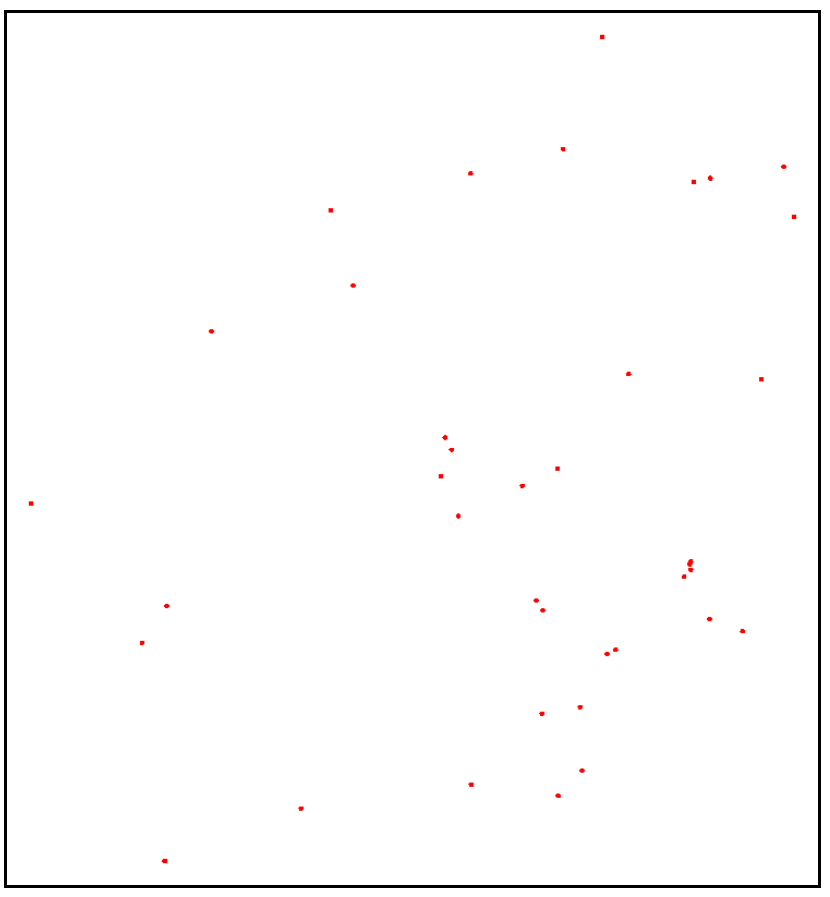
\includegraphics[width=\textwidth]{figures/world_dj38_tsp_data.png}
    \caption{Figure showing world TSP test data, the nodes form like cities on a map. This example is based on 38 cities from Djibouti. This problem came from \cite{dj38_tsp_instance}.}
    \label{fig:world_tsp_data}
\end{figure}

\section{Background}
My motivation for this project was based around my interest in Algorithms and finding new approaches to solve challenging problems, In 1991 ACO was first applied to solve TSPs\cite{dorigo1991distributed} this algorithm was called "Ant System" and was tested on several TSPs. It was able to solve TSPs of small sizes but didn't perform as well in solving larger problems. 

ACO is a probabilistic search technique which is used to find good paths through graphs. In the real world when an Ant leaves its nest to find food it initially randomly wanders, whilst it is wondering it is laying down a pheromone trail. When it finds some food it will follow its pheromone trail back to the nest but still has a chance to go off randomly. Ants aren't guaranteed to follow a trail of pheromone they can go off and randomly wonder, this is what allows the ants to find better paths between the food and their nests. ACO is based on this pheromone communication, figure \ref{fig:aco_pheremone_example} shows how an ants trail changes based on this pheromone. Over time this pheromone trail evaporates which reduces its attractiveness towards ants, the longer the path the more time it has to evaporate. A short path that gets travelled frequently will have much less evaporation because of the more ants travelling over it. This evaporation is also what leads to the ants avoiding a locally optimal solution because without it then the first path that was travelled would be the final path.

\begin{figure}
    \centering
    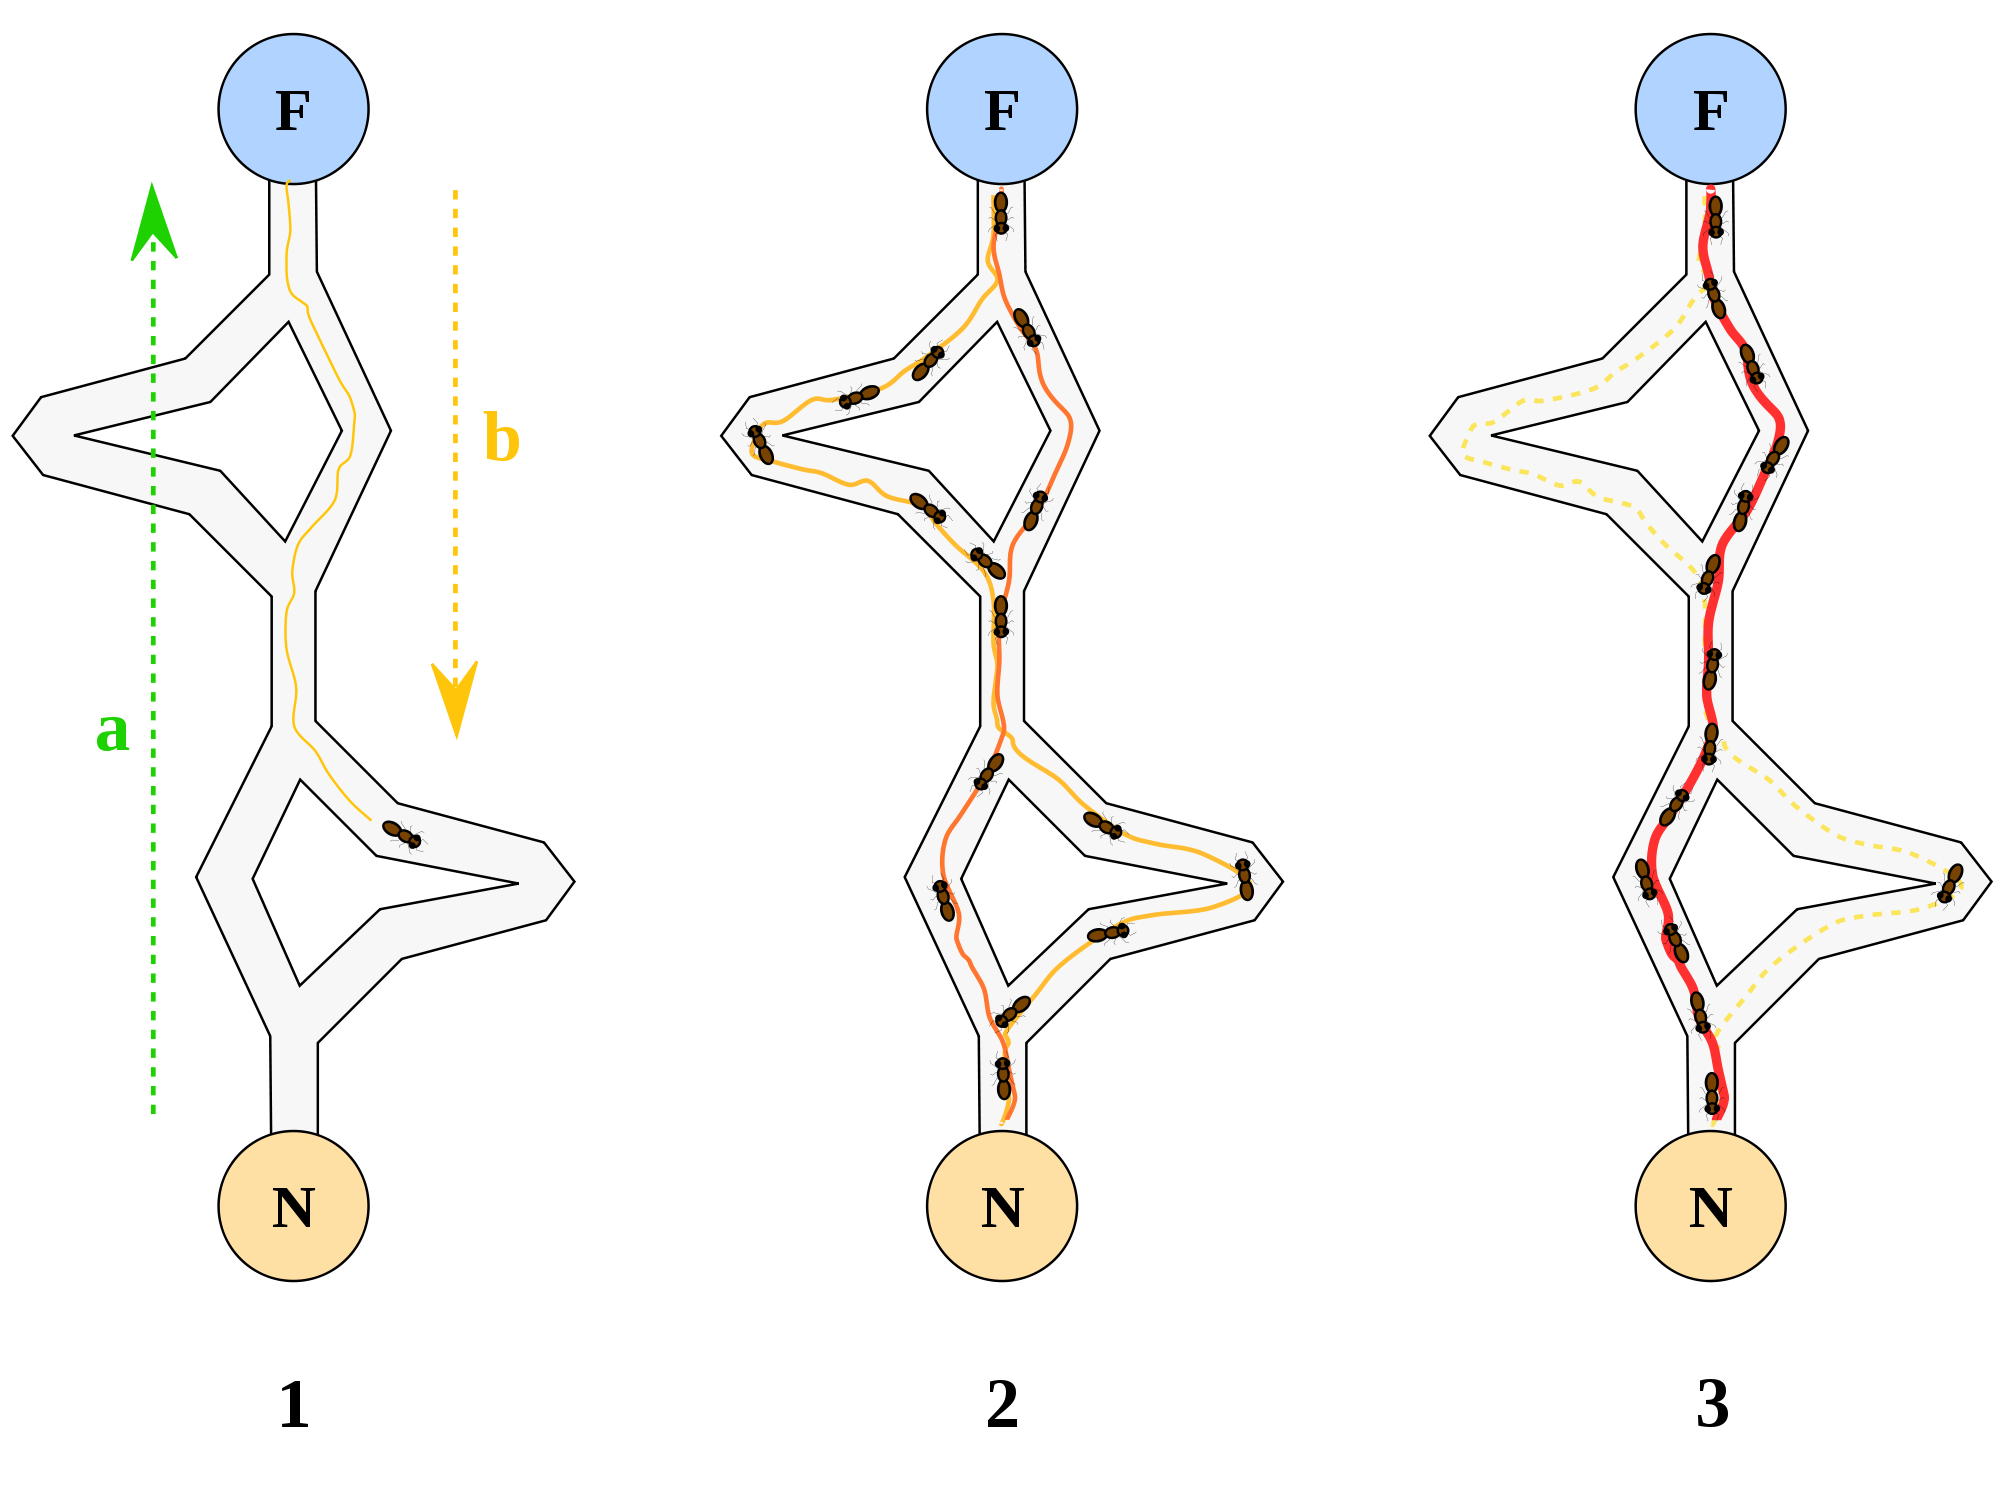
\includegraphics[width=\textwidth]{figures/aco_pheremone_demo.png}
    \caption{Figure showing how in nature ants deposit pheromone and change their paths based on the pheromone from other ants. The Ants choose a path based on the pheromone that has been deposited but there is also a random chance that the ant will choose a different route, this is what allows ACO to change routes and find a better solution.}
    \label{fig:aco_pheremone_example}
\end{figure}

There are a few key formulas that enable ACO to achieve this, the edge selection equation shown in figure \ref{eq:ACOEdgeselection} and the pheromone update equation which is shown in figure \ref{eq:pheremoneupdate}. 

\begin{figure}[h]
    \centering
    $
    p_{xy}^k =
    \frac
    { (\tau_{xy}^{\alpha}) (\eta_{xy}^{\beta}) }
    { \sum_{z\in \mathrm{allowed}_x} (\tau_{xz}^{\alpha}) (\eta_{xz}^{\beta}) }$
    \caption{This is the edge selection formula for ACO. Ant $k$ moves from state $x$ to state $y$ with this probability. $\tau_{xy}$ is the amount of pheromone deposited when transitioning from $x$ to $y$. $\alpha$ is a value equal to or greater than 0 which controls $\tau_{xy}$. $\eta_{xy}$ is how desirable that transition is, $\beta$ controls this desirability.}
    \label{eq:ACOEdgeselection}
\end{figure}

\begin{figure}[h]
    \centering
    $ \tau_{xy} \leftarrow
    (1-\rho)\tau_{xy} + \sum_{k}\Delta \tau^{k}_{xy}$
    
    $\Delta \tau^{k}_{xy} =
    \begin{cases}
    Q/L_k & \mbox{if ant }k\mbox{ uses curve }xy\mbox{ in its tour} \\
    0 & \mbox{otherwise}
    \end{cases}$
    \caption{This is the pheromone update equation. Pheromones are updated when an Ant completes its tour, the pheromones levels are increased for 'good' tours and decreased for 'bad' tours. $\tau_{xy}$ is the amount of pheromones deposited when transitioning from state $x$ to state $y$. $\rho$ is the pheromone evaporation constant, $\Delta \tau^{k}_{xy}$ is the amount of pheromone deposited by ant $k$. $Q$ is the pheromone constant value and $L_k$ is the tour length for ant $k$.}
    \label{eq:pheremoneupdate}
\end{figure}

ACO has several parameters you can tune; the number of iterations that it runs, the number of ants that are simulated, the amount of pheromone that is deposited, the amount of pheromone that evaporates each iteration, the weighting that the pheromone has on the ants decision, called the alpha value, and the weighting that the distance of the edge has on the ants decision, this is called the beta value. ACO algorithms make a choice between whether they will follow the pheromone deposits or change path and follow a heuristic, this is what the alpha and beta values are for. This allows the algorithm to be probabilistic and improve upon its tours, however because of this probabilistic nature it can produce different tours on consecutive runs. If you have a high alpha value then the ant is more likely to follow the other ants that came before it, and if you have a high beta value then the ant is more likely to choose a route that has the lowest distance. There is a balance to be struck because going to the closest node does not always result in the best overall tour.

ACO is not efficient at finding the solution for large problems because its run time is to high, it's possible to tune the parameters of the algorithm such as reducing the number of iterations it will perform however doing this could mean that it finds a worse solution. 

The main way to cut the run time of ACO is to cut down on the number of nodes. The run time of ACO is \[O(t\textsubscript{max}MN^2)\] where t\textsubscript{max} is the number of iterations, M is the number of ants and N is the number of nodes\cite{pang_chao-yang_ben-qiong_zhang_jie_wei_shan_zheng-chao_2014}. The run time is proportional to N\textsuperscript{2} so the only way to cut down the run time of the algorithm without compromising the quality of the solution is to cut down the number of nodes.

There are many different clustering algorithms available it is my goal to implement quite a few of them so that there is a choice and the different clustering algorithms can be analysed in respect to their effect on ACO. The Python library Scikit Learn\cite{scikit_learn_python_library} has implemented many different clustering algorithms\cite{scikit_clustering} and so I will be using that to do my clustering, I will choose a selection of these algorithms and should be able to compare them to see which ones perform better against ACO.

The tour that ACO produces may not be optimal because it didn't run for long enough or the parameters where not tuned correctly to fix this there is a local search algorithm called 2-opt that takes a tour created from a heuristic and attempts to improve it\cite{venhuis_2019} It improves the tour by reordering the nodes, it performs very well at removing paths in the tour that cross over each other but does not always find the optimal solution because it is bound to the tour that was found in the heuristic and simply finds the local optimum of this. 2-opt swaps two nodes to see if this improves the tour, there are other algorithms that act similarly 2.5-opt and 3-opt. These swap more nodes which can find bigger improvements.

When traversing the clustered tour there will need to be a way of going from the global clustered tour to the local inside each cluster tour. To do this there will need to be nodes assigned on each cluster that are the entry and exit nodes and then a tour will have to be made in each cluster from the entry node to the exit node. To find this tour I will implement ways of finding the solution with ACO and through a greedy nearest neighbours approach.

\section{Analysis}

\subsection{The Current State of Solving TSPs with ACO and Clustering}
As I've previously mentioned ACO has been applied to TSP many times before but this has mostly centred around using just ACO, in \cite{assesmentdiffacofortsp} different ACO algorithms are all put to work solving a particular TSP and assessed based on how quickly they take to run and how close to optimal their solution is. This paper considers five different ACO algorithms and offers a good comparison of how well suited these algorithms are to solve TSPs as well as offering good explanations of the types of ACO algorithms. 

Clustering has been used before as part of a solution to solve TSPs in \cite{clustering_with_local_search_heuristic}, in this study Clustering was used alongside a Genetic Algorithm and it showed that when clustering the data and then running the GA an improved TSP tour was found.

As briefly mentioned earlier \cite{pang_chao-yang_ben-qiong_zhang_jie_wei_shan_zheng-chao_2014} used ACO and clustering to solve TSPs and in their research they found that using clustering did speed up the ACO process they also created their own clustering algorithm the "Local Clustering Algorithm" which better expands to fit TSP data. 

The paper \cite{yang_shi_marchese_liang_2008} talks about using ACO to solve TSPs by dividing the nodes into groups and then visiting those groups. This is similar to clustering. It also uses mutation to avoid being locked into poor decisions allow the path to break out of a local minimum. It also uses 2-opt to speed up the finding of a good solution.

In \cite{10.1007/11839088_31} they create a new clustering algorithm which uses the features of ACO to group data. Existing clustering solutions converge prematurely and end up finding a local minimum this algorithm attempted to mitigate that by sending ants out along their paths and building up pheromone trails, at each step of the ants trail it selects a node that doesn't belong to a cluster and adds it to one. The ants deposit pheromones on nodes and nodes that have more pheromone are more attractive to ants. When the ants select nodes they use a combination of this pheromone and a euclidean distance heuristic. 

\subsection{Intended Approach}
There are many directions to take this project and things that I could discuss and do however because I've only got a few months to do this project I'm going to be limited. I would like to mostly look at the interactions of ACO on solving TSPs and seeing how clustering affects this.

I had to decide on the clustering algorithms that I wanted to use, as I mentioned briefly before I am using the Python library Scikit Learn to do my clustering and this implements 10 clustering algorithms. I want to choose clustering algorithms that all work in slightly different ways so that I have a better chance to find a clustering algorithm that better works for TSP data. I have selected the K-Means, Affinity Propagation, DBSCAN, OPTICS and Birch clustering algorithms. 

The K-Means algorithm splits the data up into N non-overlapping clusters each data point belongs to only one cluster, it attempts to place the clusters as far away from each other whilst also making the intra-cluster data points as similar as possible. K-means works well for a very large number of nodes and quite a lot of clusters. This algorithm is good to use because it allows the number of clusters to be specified. This particular implementation requires a parameter called 'n\_init', this value indicates the number of times the algorithm will be ran with different centroid the final result will be the run that has the best output in terms of the parameters mentioned above.

Affinity Propagation is different to the others because it works out the number of clusters there should be it does this by working out the similarities between each data point. It doesn't work very well with a large number of nodes this is because of the computation and memory resources needed to calculate the number of nodes. It requires two arguments max\_iterations and convergence\_iterations, Affinity Propagation runs in iterations and tries to converge points together into clusters. max\_iterations refers to the maximum number of iterations that will be run in total before it stops, convergence\_iterations is the number of iteration that need to happen sequentially with no change in order for the algorithm to stop. 

The next clustering algorithm I chose was DBSCAN, this chooses the number of clusters based on two values eps and min\_samples. A higher min\_samples value or a lower eps value means that a higher density is needed for a cluster to form. The min\_samples value refers to the number of nodes that need to be in a neighbourhood for that to be considered a core point and a cluster to form around it, the eps value refers to the maximum distance between two nodes for them to be considered in the same neighbourhood, it's not the maximum distance between points in a cluster if there is a dense but spread out cluster then the size of the cluster can be larger then this value. The eps value is the most important factor to choose correctly. This algorithm scales up to a large amount of nodes and quite a lot of cluster. This also supports classifying nodes as 'noise' these nodes do not fit into any cluster because they are too far away from other nodes.

I chose the OPTICS algorithm because like DBSCAN it supports classifying nodes as noise and it doesn't require the number of clusters to be set but unlike DBSCAN it doesn't require an eps value. It is very similar to DBSCAN in that it finds areas of high density but it differs in its approach to find the clusters because it generates a reach ability graph this allows it to find a sensible density value in order to build clusters. It is better suited to large datasets than DBSCAN however at the sizes that I will be examining I am unsure if this will matter. It requires a parameter called min\_samples this is the same as the parameter of the same name for DBSCAN, it affects the number of nodes that need to be together for the nodes to form into a neighbourhood.

The last clustering algorithm I chose was BIRCH, this algorithm works by building a tree for the data that you want to cluster. It requires three arguments; the branching factor, the number of clusters and a threshold value. This algorithm works well with a large number of clusters and a large number of nodes, this was the reason it was chosen.

In the time I have I will not be able to create an algorithm that can deal with massive TSPs that contain 10's of thousands of nodes or an algorithm that can necessarily find an optimal solution to every piece of data. I will instead focus on smaller problems and evaluating the results of these questions.

The questions that I propose for this project are;

\subsubsection{Does clustering allow ACO to be applied to larger problems.}

This question is about seeing how clustering impacts the run time of ACO and if clustering the data means that the run time is lower. To evaluate this question I will choose several pieces of TSP data of various sizes with both VLSI and world TSP data used, then I will have a run that does ACO only and a run that does ACO with a clustering algorithm. The run times and solution lengths will be calculated and compared. During these tests 2-opt will not be ran and the ACO parameters will stay the same for every test.

\subsubsection{To what effect do different clustering algorithms have on the quality and run time of the solution.}

This question is about seeing the change that clustering algorithms have on the solution. To run this experiment I will use the same ACO algorithm and parameters and then use different clustering algorithms to see if there is one that is particularly suited to use with TSP data. I will use TSP data of varying sizes as well as TSP that is of the VLSI type and the world type. To find the tour inside each cluster I will use both ACO and the greedy nearest neighbours approach. 

It would be interesting to see if I could create a new algorithm that can better deal with TSP data. In 'Applying Data Clustering Feature to Speed Up Ant Colony Optimization'\cite{pang_chao-yang_ben-qiong_zhang_jie_wei_shan_zheng-chao_2014} they create a new local clustering algorithm that measures the direction in which TSP data extends. This allows the clusters to better form around TSP data which should result in a better overall solution. It would be nice to implement my own clustering solution but I feel in the time I have that this may not necessarily be possible. It might be possible to improve existing clustering methods to better account for TSP data or speed up the process of clustering. 

The best kind of clustering algorithms to use will be ones that can deal with data that doesn't belong to any specific cluster, in most TSP problems there will be data that will not neatly fit into any specific cluster and this should be able to be dealt with. 

When it comes down to analysing the clustering algorithms that allow the number of clusters to be set I will vary the number of clusters.

\subsubsection{When using 2-opt with ACO and clustering what effect do the clusters have on the overall solution, does 2-opt end up finding the same solution or nearly the same solution regardless of the clustering algorithm used.}

This is about seeing how clustering really affects the final solution when 2-opt is used to smooth the solution out and find the local optimal solution, is this local optimum solution the same regardless of clustering algorithm used. This will also be able to show if there is a clustering algorithm that is superior for this application. To run this test I will keep the ACO algorithm and parameters the same and change the clustering algorithm. I will run this test on various sizes of TSP data on both world and VLSI data types. 

\subsubsection{What effect does varying the ACO parameters have on the solution.}

ACO can have a huge impact over the final solution, if the ACO run gave a bad solution then 2-opt can take longer and possibly not find as good a solution as it could of. ACO has a lot of parameters that can be tuned and it would be interesting to identifying the ones that most impact a TSP solution.

To run this experiment I would choose a world and VLSI TSP problem and a clustering algorithm. I would then vary the ACO parameters and see how these affected the quality of the solution found. I could measure this both before and after 2-opt has been ran to also see how ACO impacts the 2-opt run.